% P(S_n >= 0.2 n) for S_n binomial(n, 0.1), exact, against the Chebyshev, Hoeffding and Chernoff bounds, log scale. Generated by a short script.
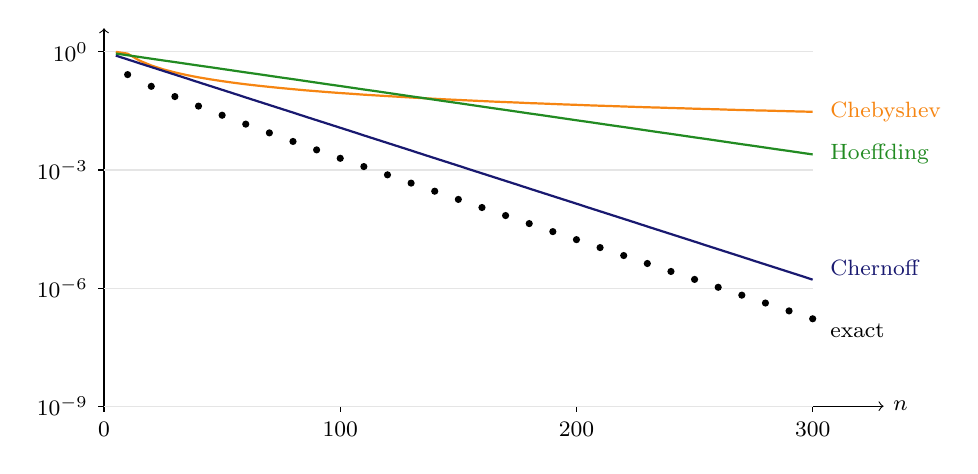
\begin{tikzpicture}
\draw[->] (0,0)--(9.90,0) node[right,font=\footnotesize] {$n$};
\draw[->] (0,0)--(0,4.80);
\draw (0.00,0)--(0.00,-0.08) node[below,font=\footnotesize] {$0$};
\draw (3.00,0)--(3.00,-0.08) node[below,font=\footnotesize] {$100$};
\draw (6.00,0)--(6.00,-0.08) node[below,font=\footnotesize] {$200$};
\draw (9.00,0)--(9.00,-0.08) node[below,font=\footnotesize] {$300$};
\draw (0,0.00)--(-0.08,0.00) node[left,font=\footnotesize] {$10^{-9}$};
\draw[black!10] (0,0.00)--(9.00,0.00);
\draw (0,1.50)--(-0.08,1.50) node[left,font=\footnotesize] {$10^{-6}$};
\draw[black!10] (0,1.50)--(9.00,1.50);
\draw (0,3.00)--(-0.08,3.00) node[left,font=\footnotesize] {$10^{-3}$};
\draw[black!10] (0,3.00)--(9.00,3.00);
\draw (0,4.50)--(-0.08,4.50) node[left,font=\footnotesize] {$10^{0}$};
\draw[black!10] (0,4.50)--(9.00,4.50);
\draw[BurntOrange,thick] plot coordinates {(0.150,4.500) (0.300,4.477) (0.450,4.389) (0.600,4.327) (0.750,4.278) (0.900,4.239) (1.050,4.205) (1.200,4.176) (1.350,4.151) (1.500,4.128) (1.650,4.107) (1.800,4.088) (1.950,4.071) (2.100,4.055) (2.250,4.040) (2.400,4.026) (2.550,4.012) (2.700,4.000) (2.850,3.988) (3.000,3.977) (3.150,3.967) (3.300,3.956) (3.450,3.947) (3.600,3.938) (3.750,3.929) (3.900,3.920) (4.050,3.912) (4.200,3.904) (4.350,3.896) (4.500,3.889) (4.650,3.882) (4.800,3.875) (4.950,3.868) (5.100,3.862) (5.250,3.856) (5.400,3.849) (5.550,3.844) (5.700,3.838) (5.850,3.832) (6.000,3.827) (6.150,3.821) (6.300,3.816) (6.450,3.811) (6.600,3.806) (6.750,3.801) (6.900,3.796) (7.050,3.792) (7.200,3.787) (7.350,3.783) (7.500,3.778) (7.650,3.774) (7.800,3.770) (7.950,3.765) (8.100,3.761) (8.250,3.757) (8.400,3.754) (8.550,3.750) (8.700,3.746) (8.850,3.742) (9.000,3.739)};
\draw[ForestGreen,thick] plot coordinates {(0.150,4.478) (0.300,4.457) (0.450,4.435) (0.600,4.413) (0.750,4.391) (0.900,4.370) (1.050,4.348) (1.200,4.326) (1.350,4.305) (1.500,4.283) (1.650,4.261) (1.800,4.239) (1.950,4.218) (2.100,4.196) (2.250,4.174) (2.400,4.153) (2.550,4.131) (2.700,4.109) (2.850,4.087) (3.000,4.066) (3.150,4.044) (3.300,4.022) (3.450,4.001) (3.600,3.979) (3.750,3.957) (3.900,3.935) (4.050,3.914) (4.200,3.892) (4.350,3.870) (4.500,3.849) (4.650,3.827) (4.800,3.805) (4.950,3.783) (5.100,3.762) (5.250,3.740) (5.400,3.718) (5.550,3.697) (5.700,3.675) (5.850,3.653) (6.000,3.631) (6.150,3.610) (6.300,3.588) (6.450,3.566) (6.600,3.545) (6.750,3.523) (6.900,3.501) (7.050,3.479) (7.200,3.458) (7.350,3.436) (7.500,3.414) (7.650,3.393) (7.800,3.371) (7.950,3.349) (8.100,3.327) (8.250,3.306) (8.400,3.284) (8.550,3.262) (8.700,3.241) (8.850,3.219) (9.000,3.197)};
\draw[MidnightBlue,thick] plot coordinates {(0.150,4.452) (0.300,4.404) (0.450,4.355) (0.600,4.307) (0.750,4.259) (0.900,4.211) (1.050,4.163) (1.200,4.114) (1.350,4.066) (1.500,4.018) (1.650,3.970) (1.800,3.921) (1.950,3.873) (2.100,3.825) (2.250,3.777) (2.400,3.729) (2.550,3.680) (2.700,3.632) (2.850,3.584) (3.000,3.536) (3.150,3.488) (3.300,3.439) (3.450,3.391) (3.600,3.343) (3.750,3.295) (3.900,3.247) (4.050,3.198) (4.200,3.150) (4.350,3.102) (4.500,3.054) (4.650,3.005) (4.800,2.957) (4.950,2.909) (5.100,2.861) (5.250,2.813) (5.400,2.764) (5.550,2.716) (5.700,2.668) (5.850,2.620) (6.000,2.572) (6.150,2.523) (6.300,2.475) (6.450,2.427) (6.600,2.379) (6.750,2.331) (6.900,2.282) (7.050,2.234) (7.200,2.186) (7.350,2.138) (7.500,2.090) (7.650,2.041) (7.800,1.993) (7.950,1.945) (8.100,1.897) (8.250,1.848) (8.400,1.800) (8.550,1.752) (8.700,1.704) (8.850,1.656) (9.000,1.607)};
\fill (0.300,4.211) circle (1.3pt);
\fill (0.600,4.062) circle (1.3pt);
\fill (0.900,3.932) circle (1.3pt);
\fill (1.200,3.811) circle (1.3pt);
\fill (1.500,3.695) circle (1.3pt);
\fill (1.800,3.582) circle (1.3pt);
\fill (2.100,3.471) circle (1.3pt);
\fill (2.400,3.362) circle (1.3pt);
\fill (2.700,3.255) circle (1.3pt);
\fill (3.000,3.148) circle (1.3pt);
\fill (3.300,3.043) circle (1.3pt);
\fill (3.600,2.938) circle (1.3pt);
\fill (3.900,2.833) circle (1.3pt);
\fill (4.200,2.730) circle (1.3pt);
\fill (4.500,2.626) circle (1.3pt);
\fill (4.800,2.523) circle (1.3pt);
\fill (5.100,2.421) circle (1.3pt);
\fill (5.400,2.319) circle (1.3pt);
\fill (5.700,2.217) circle (1.3pt);
\fill (6.000,2.115) circle (1.3pt);
\fill (6.300,2.014) circle (1.3pt);
\fill (6.600,1.913) circle (1.3pt);
\fill (6.900,1.812) circle (1.3pt);
\fill (7.200,1.711) circle (1.3pt);
\fill (7.500,1.610) circle (1.3pt);
\fill (7.800,1.510) circle (1.3pt);
\fill (8.100,1.410) circle (1.3pt);
\fill (8.400,1.310) circle (1.3pt);
\fill (8.700,1.210) circle (1.3pt);
\fill (9.000,1.110) circle (1.3pt);
\node[BurntOrange,font=\footnotesize,anchor=west] at (9.10,3.74) {Chebyshev};
\node[ForestGreen,font=\footnotesize,anchor=west] at (9.10,3.20) {Hoeffding};
\node[MidnightBlue,font=\footnotesize,anchor=west] at (9.10,1.76) {Chernoff};
\node[font=\footnotesize,anchor=west] at (9.10,0.96) {exact};
\end{tikzpicture}
